\documentclass{resume}

\usepackage{xcolor}
\begin{document}

% new command defined ---------------------------------------------
\newcommand\tab[1][1cm]{\hspace*{#1}}
\newcommand\tob[1][0.2cm]{\hspace*{#1}}
\fontfamily{ppl}\selectfont
% -----------------------------------------------------------------

% *************** PAGE - 1 ******************************************

% ======== INTRODUCTION PART ========================================

\noindent
% TOP general detais part ------------------------------------------
\begin{tabularx}{\linewidth}{@{}m{0.8\textwidth} m{0.2\textwidth}@{}}
{
	% 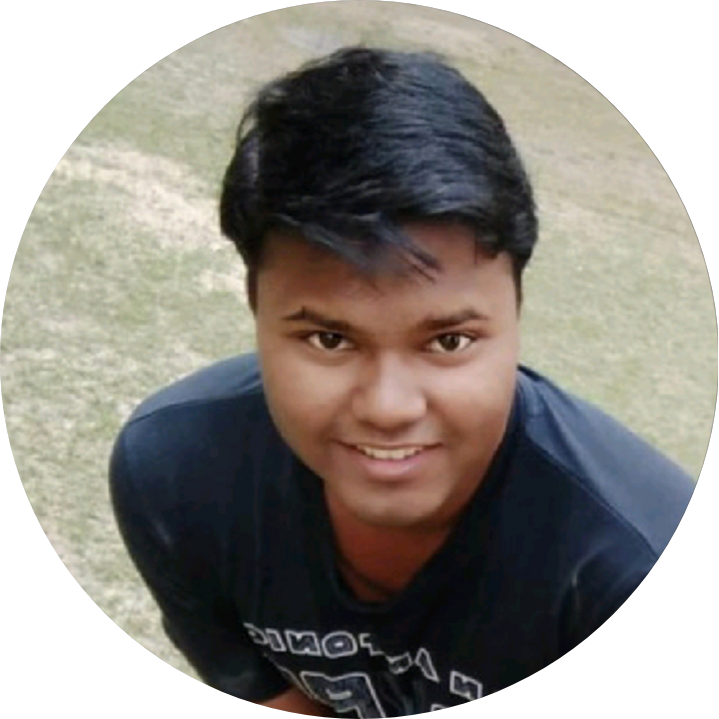
\includegraphics[width=0.6cm]{images/image3.png}
	\Large\textcolor{red}{ \textbf{Akash Ramanand Rajak}} \newline
    \small{
        \clink{
            \href{mailto:aakashrajak02@gmail.com}{\textcolor{cyan}{
\includegraphics[width=0.4cm]{images/mail.png}       \underline{aakashrajak02@gmail.com}}} \tob\textbf{|}\tob
            \href{mailto:435_bt19@iiitkalyani.ac.in}{\textcolor{cyan}{
\includegraphics[width=0.4cm]{images/mail.png}       \underline{435\_ bt19@iiitkalyani.ac.in}}}
            \newline
            {
\includegraphics[width=0.4cm]{images/phone.png} \fontdimen2\font=0.75ex \textcolor{violet}{+91 8980153352}}  \tob\textbf{|}\tob
            % \textbf{·} 
            %\href{https://johnmyweb.com}{johnmyweb.com}
        } % \newline
        
\includegraphics[width=0.4cm]{images/calender.png}
        \textcolor{violet}{D.O.B.\tob :\tob 22\tob Nov,\tob 1999}
        \newline
        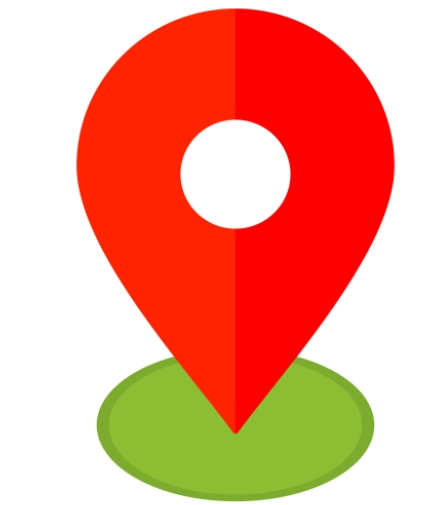
\includegraphics[width=0.4cm]{images/location.png}
        \textcolor{violet}{Gujarat,\tob India\tob  -\tob  391410}
    }
}
% ------------------------------------------------------------------

 & 

% Image Part ------------------------------------------------------
{
    \hfill
    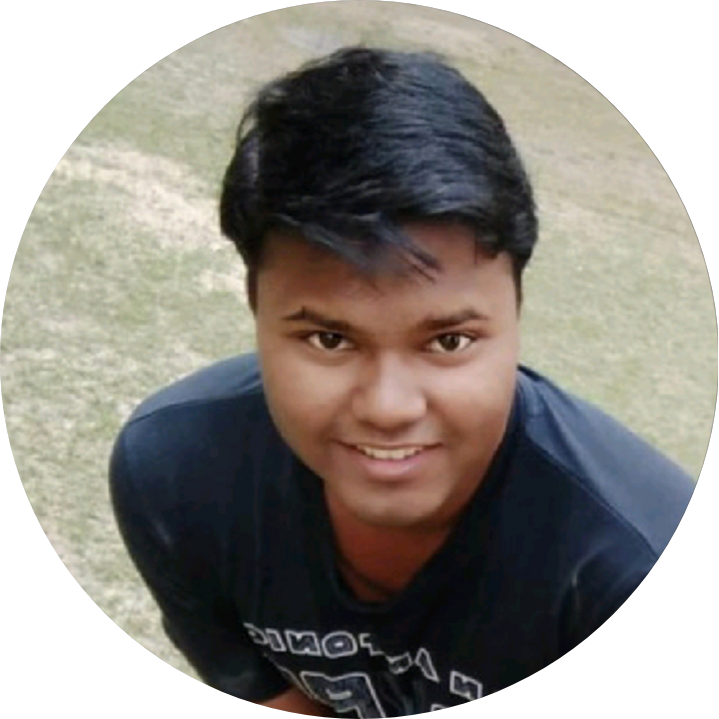
\includegraphics[width=3.0cm]{images/image3.png}
}
% -----------------------------------------------------------------
\end{tabularx}

% ===================================================================


\begin{center}
\begin{tabularx}{\linewidth}{@{}*{2}{X}@{}}
% left side %
{
	% -------- EDUCATION PART ----------------------------------
	\csection{\textcolor{blue}{EDUCATION}}{\small
        \begin{itemize}
            % item 1 %
            \item \frcontent{\textcolor{violet}{SSC}}{Gujarat Refinery English Medium School (GREMS)}{Percentile\tob :\tob 98.95\tab Grade\tob :\tob A2}{2014 - 2016}
            \item \frcontent{\textcolor{violet}{HSC - Maths, Physics, Chemistry}}{Baroda High School, Alkapuri}{Percentile\tob :\tob 92.06\tab Grade\tob :\tob B1}{2016 - 2018}
            \item \frcontent{\textcolor{violet}{B - Tech Computer Science}}{Indian Institute of Information Technology, Kalyani}{CGPA Till Sem - 4\tob :\tob 8.9029}{2019 - 2023}
        \end{itemize}
    }
    
	% -------- SKILLS PART ----------------------------------
	\csection{\textcolor{blue}{SKILLS}}{\small
        \begin{itemize}
        	\item \textbf{\textcolor{violet}{Programming Languages}} \newline
            {\footnotesize C, C++, Java, Python (Numpy, Pandas, Matplotlib, Seaborn, Tkinter, OpenCv), HTML-CSS, Scilab, MIPS Assembly Language}{}{}
            \item \textbf{\textcolor{violet}{Technologies}} \newline
            {\footnotesize Dev C++, Pycharm, Jupiter Notebook, Eclipse,  Android Studio, Scilab, Qtspim, Git \& Github, NLP, ML}{}{}
            
            \item \textbf{\textcolor{violet}{Languages}} \newline
            {\footnotesize English,  Hindi,  Gujarati}
        \end{itemize}
    }    
    
    % -------- EXPERIENCE PART ----------------------------------
   	\csection{\textcolor{blue}{EXPERIENCE}}{\small
        \begin{itemize}
            \item \frcontent{\textcolor{violet}{Winter Of Code - Student Member}}{Developer Student Club - IIIT Kalyani}{-\tob   Mentored by\tob :\tob Omkar Ajnadkar\newline -\tob Project\tob :\tob Tabular ML (Built an end-to-end ML system for tabular datasets).\newline -\tob  Participated in Android Study Jam.}{\tob  JAN 2021 - MAR 2021\tob (3 mos)}
        \end{itemize}
        \begin{itemize}
            \item \frcontent{\textcolor{violet}{LGM SOC'21 - Open Source Contributor}}{Lets Grow More}{}{\tob  JUN 2021 - Present\tob}
        \end{itemize}
    }
    
} 
% end left side %
& 
% right side %
{
    % -------- PROJECTS PART ----------------------------------
    \csection{\textcolor{blue}{PROJECTS}}{\small
        \begin{itemize}
            % PROJECT - 1 ----------------
            \item \frcontent{\textcolor{violet}{CaveMan\tob -\tob The\tob Saviour} \clink{\href{https://github.com/akash435/CaveMan-The_Saviour}{\tob \textcolor{cyan}{\underline{[Github\tob Link]}}}}}{-\tob A 2D physics-based game app created with Android Studio and with simple graphics.}{-\tob It is an enemy killing game, where player need to reach the winning score by killing the enemies.\newline -\tob The game is also split in different level, making player to challenge different stages of enemy.}{+\tob Features used - Java, Android, Sqlite database}
            
            % PROJECT - 2 ----------------
            \item \frcontent{\textcolor{violet}{PasswordStrengthPredictor} \clink{\href{https://github.com/akash435/Password-Strength-Predictor}{\tob \textcolor{cyan}{\underline{[Github\tob Link]}}}}}{-\tob Built a NLP and ML model, to predict the strength of passwords, using csv dataset.}{-\tob Used nltk library for for NLP and numpy, pandas module for preprocessing purpose.\newline- \tob Used different models like Linear Regression, Ridge Regression, Decision Tree Regressor for better accuracy.}{+\tob Features used - Python(Numpy, Pandas, Seaborn), Logistic Regression, Jupiter Notebook}
            
            % PROJECT - 3 ----------------
            \item \frcontent{\textcolor{violet}{Dictionary} \clink{\href{https://github.com/akash435/Dictionary}{\tob \textcolor{cyan}{\underline{[Github\tob Link]}}}}}{-\tob Built an English dictionary using tkinter GUI.}{-\tob For data set, used JSON data file.\newline -\tob Also implemented the case of word having interfaces (many meanings) and in case of any typo, developed the closest word matching technique.\newline -\tob Also implemented the auto-complete feature.}{+\tob Features used - Python (json, Tkinter)}
            
            % PROJECT - 4 ----------------
            \item \frcontent{\textcolor{violet}{Simple Python IDE} \clink{\href{https://github.com/akash435/Dictionary}{\tob \textcolor{cyan}{\underline{[Github\tob Link]}}}}}{-\tob Built a  Simple Python IDE using tkinter GUI.}{-\tob Here User will be able to run python code and see the output by running it.\newline -\tob Added feature to change the mode of coding area to black mode.\newline -\tob Also implemented the auto-complete feature.}{+\tob Features used - Python (Tkinter, StringIO)}
        \end{itemize}
    }
    
}
\end{tabularx}
\end{center}
% ********************************************************************

% *************** PAGE - 2 ******************************************

\begin{center}
\begin{tabularx}{\linewidth}{@{}*{2}{X}@{}}
% left side %
{
    % -------- COURSES PART ----------------------------------
    \csection{\textcolor{blue}{COURSES}}{\small
        \begin{itemize}
            \item \textbf{\textcolor{violet}{Mathematics}} \newline
            {\footnotesize Linear Algebra, Probability and Statistics, Dicrete Mathematics, Calculus and Differential Equation, Numerical Analysis and Computing}{}{}
            \item \textbf{\textcolor{violet}{Computer Science}} \newline
            {\footnotesize Programming with C, Data Structures and Algorithm, Algorithm Analysis and Design, Computer Architecture, Formal Language and Automata Theory, Data Science (Python), Operating System, Object Oriented Programming (JAVA), Scilab, Qtspim}
            \item \textbf{\textcolor{violet}{Electronics}} \newline
            {\footnotesize Digital Electronics, Analog Electronics, Data Communication, Signals and Systems}
            \item \textbf{\textcolor{violet}{Others}} \newline
            {\footnotesize Physics, Ethics, Economics, Humanity (Psychology)}
        \end{itemize}
    }
    
    \csection{\textcolor{blue}{Interests \& Hobbies}}{\small
        \begin{itemize}
            \item {\footnotesize Competitive Programming\tab \textbf{•} \tob Open Source}
        \end{itemize}
    }
    % -------- LINKS PART ----------------------------------
	\csection{\textcolor{blue}{LINKS}}{\small
        \begin{itemize}
            \item 
            \clink{
        	\href{https://github.com/akash435}{\textcolor{cyan}{
\includegraphics[width=0.4cm]{images/github.png}\tob   \underline{Github}}}
        	\textbf{} 
        	\href{https://www.linkedin.com/in/akash-rajak-akash435/}{\textcolor{cyan}{
\includegraphics[width=0.4cm]{images/linkedin.png}\tob \underline{Linkedin}}}
        	\textbf{}
        	\href{https://www.hackerrank.com/aakashrajak02?hr_r=1}{\textcolor{cyan}{
\includegraphics[width=0.4cm]{images/hackerrank.png}\tob \underline{HackerRank}}}
        }
        \end{itemize}
        
        \begin{itemize}
            \item 
            \clink{
        	\href{https://www.codechef.com/users/akash435}{\textcolor{cyan}{
\includegraphics[width=0.4cm]{images/codechef.png}\tob \underline{CodeChef}}}
        	\textbf{}
        	\href{https://codeforces.com/profile/aakashrajak02}{\textcolor{cyan}{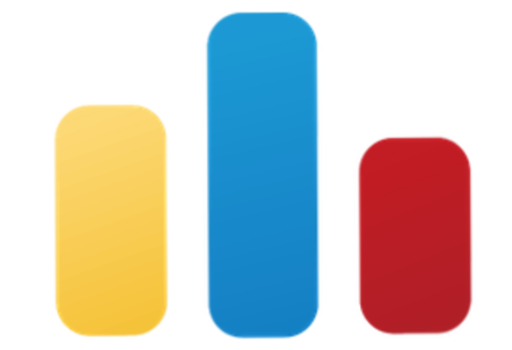
\includegraphics[width=0.4cm]{images/codeforces.png}\tob \underline{Codeforces}}}
        	\textbf{}
        	\href{https://leetcode.com/akash435/}{\textcolor{cyan}{
\includegraphics[width=0.4cm]{images/leetcode.png}\tob \underline{LeetCode}}}
            %\newline
        }
        \end{itemize}
    }
    
} 
% end left side %
& 
% right side %
{
	% -------- EVENTS & PARTICIPATIONS PART ----------------------------------
    \csection{\textcolor{blue}{Events \& Participations}}{\small
        \begin{itemize}
            \item {\footnotesize Participated in Google Coding Competition - HashCode 2021, CodeJam 2021, KickStart 2021.}
            \item {\footnotesize Participated in Devfolio Hackathon HackData 5.0, with project BSM.}
            \item {\footnotesize Participated in Code Kaze'21, Code Frenzy - Online Coding Competion by Coding Ninjas.}
        \end{itemize}
    }
    
    % -------- CERTIFICATIONS & AWARDS PART ----------------------------------
    \csection{\textcolor{blue}{Certifications \& Awards}}{\small
        \begin{itemize}
            \item 
            \clink{
        	\href{https://drive.google.com/file/d/10sXwmb6wxSuvKRxmuy-zUPSzIliKLoce/view}{\textcolor{cyan}{\underline{Code Kaze'21}}}
        	\tob
        	\textbf{|} 
        	\tob
        	\href{https://drive.google.com/file/d/1yKLWfopv5k2C1YMbC8GmZNl1wXWj2vXq/view}{\textcolor{cyan}{\underline{Code Frenzy}}}
        }
        \end{itemize}
        
        \begin{itemize}
            \item 
            \clink{
        	\href{https://drive.google.com/file/d/11pssUHnwQSHhpv3muc3RsOlsujGNo9Zt/view}{\textcolor{cyan}{\underline{Android Study Jam}}}
        	\tob
        	\textbf{|} 
        	\tob
        	\href{https://drive.google.com/file/d/1LdR-E4uXdbXYD3yLiHGOtKpeYbjZcNo6/view}{\textcolor{cyan}{\underline{Winter Of Code}}}
        }
        \end{itemize}
    }
}
\end{tabularx}
\end{center}

% *******************************************************************

\end{document}\
